% !TEX encoding = UTF-8
% !TEX TS-program = pdflatex
% !TEX root = ../tesi.tex

%**************************************************************
\chapter{Theoretical basis}
\label{cap:theoretical-basis}
%**************************************************************

\section{Signals and modulation}

Modern wireless communication systems are usually analyzed using a \emph{baseband equivalent representation}, where passband signals are expressed in terms of their complex envelope. A transmitted signal can be written as:

\begin{equation}
    s(t) = \Re \{ x(t) e^{j 2 \pi f_c t} \}
\end{equation}
where $x(t)$ is the complex baseband signal and $f_c$ is the carrier frequency. This representation separates the information bearing component from the carrier.\\
Digital communication systems map discrete symbols onto complex values in a constellation diagram. Common modulation schemes include\gls{PSK}, where each symbol corresponds to a point in the complex plane. At the receiver, detection consists of identifying the transmitted symbol on the basis of the received signal's position relative to predefined decision regions \cite{oppenheim1996signals}.

\begin{figure}[htbp]
    \centering
    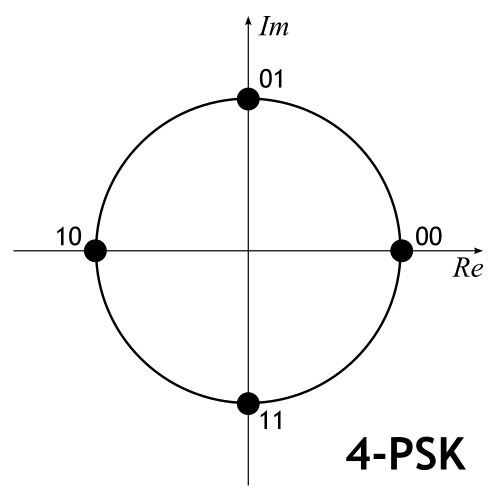
\includegraphics[width=0.5\textwidth]{images/chapter2/4psk_constellation_example.png}
    \caption{Example of mapping of 4 symbols to a constellation diagram. Source \cite{superspritz2025qpsk}}
    \label{fig:4psk_constellation_example}
\end{figure}



\section{Antenna arrays}
An antenna array consists of multiple radiating elements arranged in space and driven with controlled amplitudes and phases; The collective radiation pattern of the array is determined by the superposition of the fields generated by each element. A key element is the \emph{array factor}, which describes how the geometry and excitation of the array shape the radiated field. For a\gls{ULA} with $N$ elements and iter-element spacing $d$, the array factor can be expressed as:

\begin{equation}
    AF(\theta) = \sum_{n=0}^{N-1} w_n e^{j n k d \sin\theta}
\end{equation}
where $w_n$ are complex weights and $k = \frac{2\pi}{\lambda}$ is the wavenumber.\\
By correctly choosing the weights $w_n$, the array can produce constructive interference in desired directions and destructive interference elsewhere, enabling spatial selectivity \cite{balanis2005antenna}.

\section{Beamforming}

Beamforming is the process of shaping the radiation pattern of an antenna array to enhance signal transmission or reception in specific directions; This is achieved by applying complex weights to the array elements, effectively steering the beam toward a desired angle. For a signal arriving from direction $\theta$, the array response can be described by a \emph{steering vector}:
\begin{equation}
    \mathbf{a}(\theta) = \begin{bmatrix}
1 & e^{j k d \sin\theta} & \cdots & e^{j (N-1) k d \sin\theta}
\end{bmatrix}^T.
\end{equation}
Beamforming consists of selecting a weight vector $\mathbf{w}$ such that the array output:
\begin{equation}
    y = \mathbf{w}^H \mathbf{x}
\end{equation}
enhances signals from a desired direction while suppressing others.
%**************************************************************
\section{Directional modulation}
\label{sec:directional_modulation}

\gls{DM} is a technique that can be implemented in various ways, but in each of them the primary focus is determining the array weights $\mathbf{w} \in \mathbb{C}^{N_t \times 1}$ that ensure standard signal transmission at Bob's side as:
\[
\begin{aligned}
    \mathcal{W}_1 &= \left\{ \mathbf{w} \ \middle|\ \mathbf{h}^H_B \mathbf{w} = s_1 \right\} \\
    \mathcal{W}_2 &= \left\{ \mathbf{w} \ \middle|\ \mathbf{h}^H_B \mathbf{w} = s_2 \right\} \\
    &\vdots \\
    \mathcal{W}_M &= \left\{ \mathbf{w} \ \middle|\ \mathbf{h}^H_B \mathbf{w} = s_M \right\}
\end{aligned}
\tag{4}
\]
where $\mathbf{h}_B \in \mathbb{C}^{N_t \times 1}$ is the channel of Bob, modeled by the array response between Alice and Bob. The subscript $1, 2, \dots, M$ represents the index of the $M$-order\gls{APM} symbol. Here, we omit the array type dependence for the notational generality of Bob's channel $\mathbf{h}_B$.
Taking the $m$th\gls{APM} symbol $s_m$ for instance and supposing the array weight set is $\mathcal{W}_m = \{\mathbf{w}^m_1, \mathbf{w}^m_2, \dots, \mathbf{w}^m_i, \cdots \}$, the transmitter has the option to consistently select $\mathbf{w}^m_i$ as the array weight for transmitting $s_m$, or randomly pick one from the array weight set $\mathcal{W}_m$ for each transmission of $s_m$. The former is referred to as static\gls{DM}, while the latter is known as dynamic\gls{DM} \cite{chen2025survey}.

\section{Physical layer security}
\label{sec:physical_layer_security}

\gls{PLS} exploits the spatial and randomness properties of the wireless channel to provide secrecy without relying on cryptographic key exchange. The foundational model is the Gaussian wiretap channel \cite{wyner1975wiretap}, in which a transmitter (Alice) communicates with a legitimate receiver (Bob) in the presence of a passive eavesdropper (Eve). The secrecy capacity of this channel is:
\begin{equation}
    C_s = \max(C_B - C_E,\; 0)
\end{equation}
where $C_B$ and $C_E$ are the Shannon capacities of the Alice--Bob and Alice--Eve links respectively. Positive secrecy capacity is achievable whenever the legitimate channel is stronger than Eve's.
Directional modulation provides a spatial mechanism to enforce this condition: the array weights are designed so that the constellation received by Bob is undistorted and decodable, while the constellation received by Eve is scrambled by phase rotations and amplitude variations that make symbol detection unreliable.

\section{Problem formulation}

\subsection{System model}
\label{sec:system_model}

Let us consider a\gls{ULA}, located on the $yz$-plane, and composed by $N$ antennas, whose locations can be expressed with Cartesian coordinates:
\begin{equation}
    \mathbf{u}_n = \begin{bmatrix}
    0 \\
    d \cdot n \\
    0
    \end{bmatrix}
    \label{eq:ULA_antenna_location_coordinates}
\end{equation}
where $n = 0, \ldots, N-1$, and $d$ is the uniform spacing across adjacent antennas. For a given set of phases $\boldsymbol{\psi} = [\psi_0, \ldots, \psi_{N-1}]^T$, the steering vector is given by:
\begin{equation}
    \mathbf{a}(\theta, \varphi) = \begin{bmatrix}
    \exp\{j\psi_0\}, & \exp\{j\psi_1\}, & \ldots, & \exp\{j\psi_{N-1}\}
    \end{bmatrix}^T
    \label{eq:ULA_steering_vector}
\end{equation}\\
The (deterministic) channel of the\gls{ULA} with respect to a wave, with wavelength $\lambda$,
impinging it under the azimuth angle $\varphi$ and elevation angle $\theta$, is:
\begin{equation}
    \mathbf{v}(\theta, \varphi) = \begin{bmatrix}
    \exp\{j\mathbf{k}^T(\theta, \varphi)\mathbf{u}_0\}, &
    \exp\{j\mathbf{k}^T(\theta, \varphi)\mathbf{u}_1\}, &
    \ldots, &
    \exp\{j\mathbf{k}^T(\theta, \varphi)\mathbf{u}_{N-1}\}
    \end{bmatrix}^T
    \label{eq:ULA_deterministic_channel}
\end{equation}
where:
\begin{equation}
    \mathbf{k}(\theta, \varphi) = \frac{2\pi}{\lambda} \cdot \begin{bmatrix}
    \cos\theta \cos\varphi \\
    \cos\theta \sin\varphi \\
    \sin\theta
    \end{bmatrix}
    \label{eq:ULA_wave_vector}
\end{equation}
is the wave vector.\\
The normalized array response of the\gls{ULA} is then given by:
\begin{equation}
    f(\theta, \varphi) = \frac{1}{N} \, \mathbf{a}^H(\theta, \varphi) \, \mathbf{v}(\theta, \varphi)
    = \frac{1}{N} \sum_{n=0}^{N-1} \exp\left\{j\left[\mathbf{k}^T(\theta, \varphi)\mathbf{u}_n - \psi_n\right]\right\}
    \label{eq:ULA_normalized_array_response}
\end{equation}\\
An example of the amplitude response $|f(\theta, \varphi)|$ and the phase response
$\angle f(\theta = 0, \varphi)$, using $N = 5$, $d = \lambda/2$, as a function of $\varphi$,
for $\theta = 0$, is reported for a random phase vector $\boldsymbol{\psi}$ in
\figurename~\ref{fig:amplitude_response} and\figurename~\ref{fig:phase_response}, respectively, using dashed lines.
Let us suppose to select the phases for each antenna such that the\gls{ULA} maximizes its response towards a specific direction $(\theta^\star, \varphi^\star)$, thus adopting the classical beamforming approach:
\begin{equation}
    \psi^\star_n = \mathbf{k}(\theta^\star, \varphi^\star) \mathbf{u}_n, \quad n = 0, \ldots, N-1
    \label{eq:ULA_beamforming_approach}
\end{equation}
In this case, $f(\theta = 0, \varphi)$ computed as in \equationname~\ref{eq:ULA_normalized_array_response}, using the optimal set of antenna phases $\boldsymbol{\psi}^\star = \{\psi^\star_n\}_{n=0}^{N-1}$ according to \equationname~\ref{eq:ULA_beamforming_approach}, assuming $\theta^\star = 0$ and $\varphi^\star = -20^\circ$ is reported in \figurename~\ref{fig:amplitude_response} (amplitude) and \figurename~\ref{fig:phase_response} (phase) using solid lines. As can be seen, the optimal antenna phases yield both the maximum gain and a null phase when $\theta = \theta^\star$ and $\varphi = \varphi^\star$.\\
Using \equationname~\eqref{eq:ULA_beamforming_approach}, \equationname~\eqref{eq:ULA_normalized_array_response} can be written in a closed form as follows:
\begin{equation}
f(\theta, \varphi) = \frac{1}{N}
\frac{\sin \left[ \pi N (\cos\theta \sin\varphi - \cos\theta^\star \sin\varphi^\star) d/\lambda \right]}
{\sin \left[ \pi (\cos\theta \sin\varphi - \cos\theta^\star \sin\varphi^\star) d/\lambda \right]}
\end{equation}


\begin{figure}[htbp]
    \centering
    \subfloat[Amplitude response $|f(\theta, \varphi)|$ \label{fig:amplitude_response}]{
        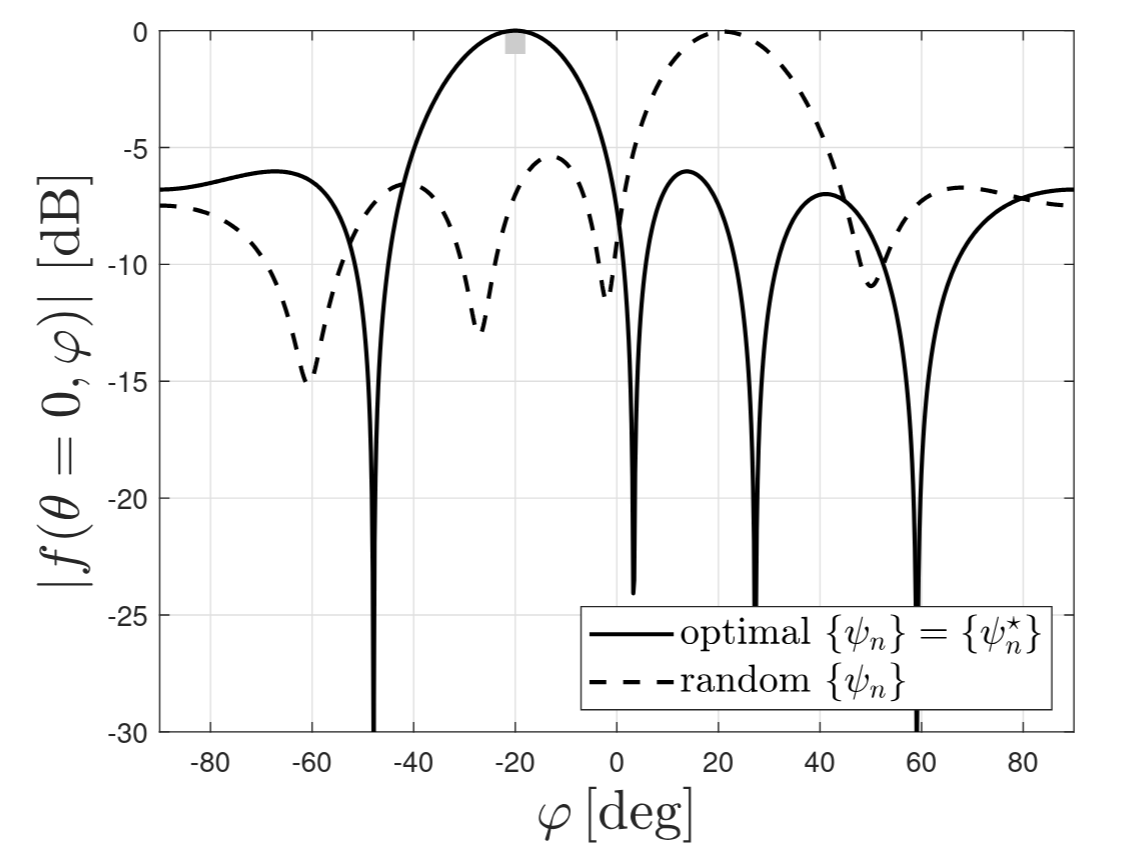
\includegraphics[width=0.8\textwidth]{chapter2/amplitude_array_response_of_ULA.png}
    }
    \vspace{0.8cm}
    \subfloat[Phase response $\angle f(\theta = 0, \varphi)$ \label{fig:phase_response}]{
        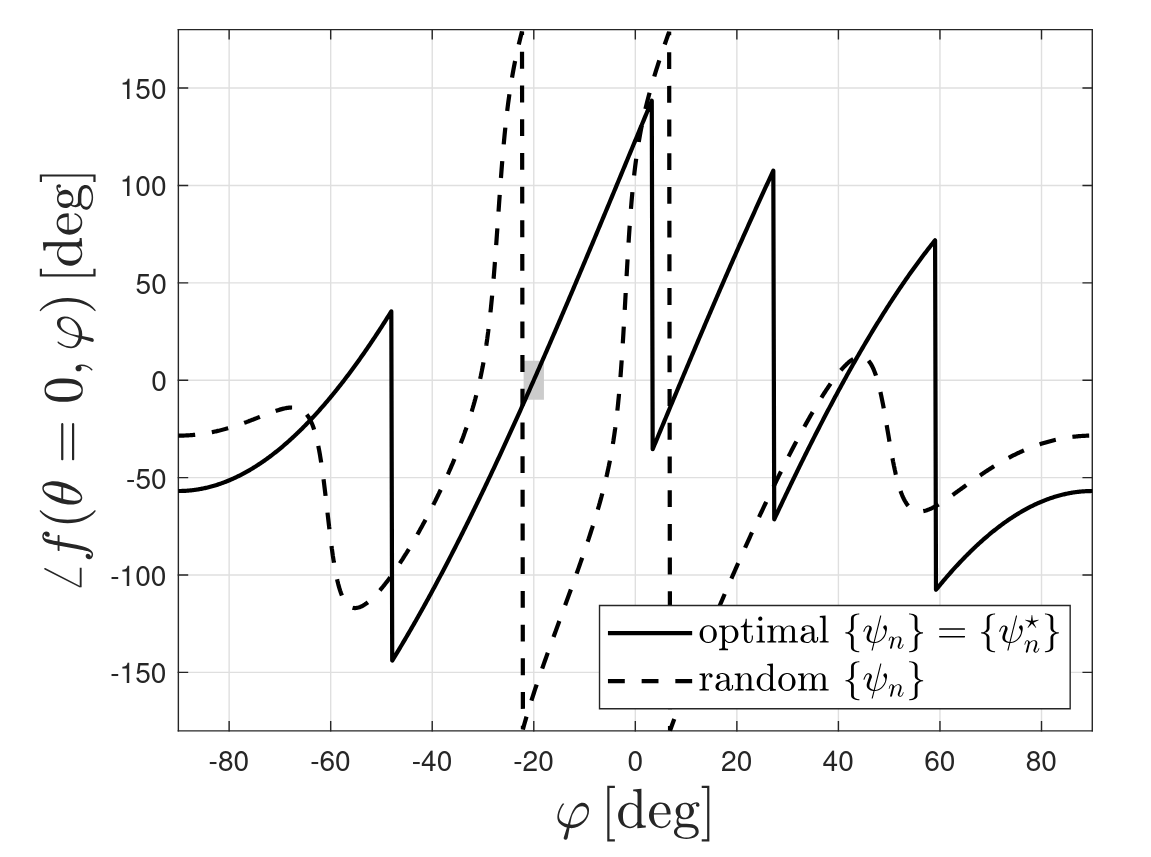
\includegraphics[width=0.8\textwidth]{chapter2/phase_array_response_of_ULA.png}
    }
    \caption{Example of the array response using $N = 5$, $d = \lambda/2$,
             for $\theta = 0$, with random $\boldsymbol{\psi}$}
    \label{fig:array_response_example}
\end{figure}

%**************************************************************


\subsection{Problem formulation}

Given the parameters introduced in \sectionname~\ref{sec:system_model}, we intend to identify an efficient
and scalable algorithm to identify acceptable realizations of $\boldsymbol{\psi}$, such that, in a
given support $[\theta^\star \pm \Delta\theta] \times [\varphi^\star \pm \Delta\varphi]$ (e.g., $\Delta\theta = \Delta\varphi = 1^\circ$):
\begin{enumerate}
    \item the amplitude $|f(\theta, \varphi)|$ satisfies the absolute floor
    $\log_{10} |f(\theta, \varphi)| \geq \varepsilon_a$
    (e.g., $\varepsilon_a = -0.7$, i.e.\ $|f| \geq 0.20$);
    \item the phase $\angle f(\theta, \varphi)$ is such that
    $|\angle f(\theta, \varphi) - \angle f(\theta^\star, \varphi^\star)| \leq \varepsilon_p$
    (e.g., $\varepsilon_p = 5^\circ$).
\end{enumerate}
To better visualize the problem, \figurename~\ref{fig:amplitude_response} and \figurename~\ref{fig:phase_response} also report the acceptable regions, obtained assuming $\Delta\varphi = 2^\circ$, $\varepsilon_a = -1\,\text{dB}$, and $\varepsilon_p = 10^\circ$, as shaded gray areas. Note that here, for simplicity, we only observe along a specific $\theta$ (namely, $\theta = 0^\circ$), which yields acceptable regions as rectangles. In general, when looking at the full support $[\theta^\star \pm \Delta\theta] \times [\varphi^\star \pm \Delta\varphi]$, acceptable regions become parallelepipeds.\\
To avoid extensive-search approaches, we can use\gls{RL} methods that draw a random realization $\boldsymbol{\psi}$, and then vary the values of the components $\psi_n$ to drive the array response to possibly fall within the acceptable regions (and hence declare $\boldsymbol{\psi}$ as a ``good'' antenna phase shift set).

\section{Reinforcement Learning}
\label{sec:reinforcement_learning}

\subsection{Reinforcement Learning and alternatives}
The problem of identifying valid beamforming configurations admits no closed-form solution in the general case, and the set of feasible phase-amplitude vectors forms a non-convex, high-dimensional region whose structure is not known a priori.
\begin{itemize}
    \item The configuration must be recovered at the symbol rate, ruling out per-instance optimization with budgets in the seconds/minutes range;
    \item The method must generalize across target directions $\varphi^\star$ without retraining or restarting;
    \item To support\gls{DDM}, repeated inferences at the same target direction must yield distinct valid configurations drawn from a sufficiently diverse distribution, so that the signal observed by an eavesdropper outside the protected angular region remains stochastic.
\end{itemize}
These requirements are most naturally framed as a demand for amortized optimization over a distribution of valid configurations: the cost of searching the feasible set is paid once, offline, in exchange for constant-time stochastic inference at deployment. The remaining design question is how to perform that amortization while preserving sample diversity.
\subsubsection{Derivative-free methods}
Derivative-free methods such as\gls{CMAES} or\gls{BO} solve the problem for a single target angle but offer no mechanism for transfer, and converge to point solutions rather than distributions. Each new $\varphi^\star$ requires a fresh search, with wall-clock costs incompatible with symbol-rate updates, and each search yields a single configuration. A natural amortization strategy is therefore \emph{supervised distillation}: run a derivative-free solver across a grid of target angles, collect the solutions, and train a regression model $\varphi^\star \mapsto (\boldsymbol{\psi}, \boldsymbol{\alpha})$. This approach was considered and rejected:
\begin{itemize}
    \item The feasible set is non-convex and multimodal in $\varphi^\star$: nearby target directions may admit valid configurations in disconnected regions of action space, and a regression model trained to interpolate between them will produce invalid outputs in the gaps;
    \item The supervised model inherits whatever biases the offline solver exhibits without any mechanism to discover better solutions than the labels it was given;
    \item A regression model is deterministic by construction: identical contexts produce identical actions, precluding the per-symbol diversity that dynamic modulation requires. Post-hoc injection of noise around a single learned point does not recover diversity over the feasible set, since perturbations of a valid configuration generally leave the feasible region given its disconnected structure.
\end{itemize}
Generative modeling of the feasible set (e.g. diffusion models) avoids the regression-interpolation problem by learning to sample from the distribution of valid configurations rather than predict a single output per angle and as such it is naturally aligned with the diversity requirement. This approach is viable in principle, but it requires a labeled dataset of valid configurations stratified by target direction, which inherits the same offline-solver bottleneck as supervised distillation. It also separates feasibility from performance: a generative model trained by maximum likelihood concentrates on the most common valid configurations, not the highest-performing or maximally diverse ones, and provides no optimization signal to shape the sampled distribution toward either security or beamforming quality.
\subsubsection{Gradient-based optimization}
Gradient-based optimization with a differentiable surrogate for the constraint check is a further alternative that, where the constraint structure admits a useful relaxation, can prove to be effective. In our setting, however, the validity condition must hold pointwise over a continuous angular support: both amplitude and phase must satisfy their respective bounds for all $(\theta, \varphi) \in [\theta^\star \pm \Delta\theta] \times [\varphi^\star \pm \Delta\varphi]$. A smooth surrogate evaluated at a finite sample of that region does not certify feasibility at unsampled points, and tightening the approximation by increasing sampling density leads to a non-smooth limit. Log-barrier formulations additionally require iterates to remain strictly feasible throughout optimization, an assumption that fails when configurations are initialized at random. These methods also produce point solutions rather than distributions, requiring a separate mechanism to recover the diversity needed for dynamic modulation. For these structural reasons, gradient-based relaxations are ill-suited to this constraint geometry.
\subsubsection{Contextual bandit}
The contextual bandit formulation directly targets amortized optimization over a distribution of valid configurations without requiring a labeled dataset. At each episode the agent observes a context $c = [\cos\varphi^\star, \sin\varphi^\star, \rho_c]$, where $\rho_c \in [0,1]$ is the curriculum constraint progress, outputs an action $\mathbf{a} = [\boldsymbol{\psi}, \boldsymbol{\alpha}] \in \mathbb{R}^{2N}$ via a stochastic policy $\pi_\theta(\mathbf{a} \mid c)$, and receives a scalar reward $r(\mathbf{a}, c)$ measuring constraint satisfaction and beamforming quality; The episode terminates after a single step \cite{lattimore2020bandit}. The reward does not need to be differentiable; the policy gradient is estimated from samples, and the stochasticity of $\pi_\theta$ serves a dual role: it drives exploration over the continuous action space during training, and at deployment it provides the per-symbol diversity required for dynamic modulation, with each forward pass sampling a fresh valid configuration from the learned conditional distribution.\\
\\
In this work,\gls{PPO} is adopted as the policy gradient algorithm using the contextual bandit formulation. Its clipped surrogate objective bounds the policy update at each gradient step, preventing destructive updates during the high-variance early phases of training when the policy has not yet identified any feasible region \cite{schulman2017ppo}.\gls{CL} is applied to stabilize convergence by ensuring the agent receives a positive reward signal before the full constraint set and training angles are enforced as expanded in \subsubsectionname~\ref{subsubsec:curriculum_learning}.

\subsection{Probability theory and stochastic processes}
\gls{RL} problems are inherently stochastic as both the system evolution and the rewards may be subject to randomness. A random variable $X$ is a mapping from an outcome space to the real numbers, and its behavior is characterized by a probability distribution.\\
A key concept is the expected value which represents the average outcome of a random variable: $\mathbb{E}[X]$.
It is also often necessary to consider conditional expectations, such as $\mathbb{E}[X \mid Y]$ which describes the expected value of $X$ given knowledge of another variable $Y$. We can now define random process as a collection of random variables indexed by time, $\{X_t\}_{t \geq 0}$ used to model systems that evolve under uncertainty. In this context, both the system state and the observed rewards can be modeled as stochastic processes \cite{ross2019probability}.

\subsection{Objective functions}
\gls{RL} can be formulated as an optimization problem over time. The performance of a decision-making strategy is quantified through a cumulative reward, defined as:
\begin{equation}
    G_t = \sum_{k=0}^{\infty} \gamma^k R_{t+k}
\end{equation}
where $R_t$ is the reward at time $t$ and $\gamma \in [0,1)$ is the discount factor which determines the relative importance of immediate and future rewards.\\
The objective is to maximize the expected return $\mathbb{E}[G_t]$. In the contextual bandit formulation used in this work, each episode consists of a single step and terminates immediately, so the sum collapses to $G_t = R_t$: the discount factor becomes irrelevant and the agent maximises expected immediate reward directly.

\subsection{Markov property}
To make sequential decision problems manageable it is often assumed that the system satisfies the \emph{Markov property}. A stochastic process $\{S_t\}$ is defined as Markovian if the conditional distribution of the next state depends only on the current state:
\begin{equation}
    P(S_{t+1} \mid S_t, S_{t-1}, \dots, S_0) = P(S_{t+1} \mid S_t)
\end{equation}
This assumption implies that the current state contains all the relevant information needed to predict the future evolution of the system, consequently, it is not necessary to retain the full history of past states.\gls{MDP} provides a formal framework for\gls{RL}.

\subsection{Policy Gradient Methods}
In problems involving continuous action spaces, it is convenient to represent the policy using a parametric function. Let $\pi_\theta(a \mid s)$ denote a policy parameterized by a vector $\theta \in \mathbb{R}^d$; The objective is to find the parameters $\theta$ that maximize the expected return:
\begin{equation}
    J(\theta) = \mathbb{E}_{\pi_\theta}[G_0]
\end{equation}
In constrast with value-based methods, policy gradient methods optimize the policy parameters directly enabling a natural treatment of stochastic policies and continuous action spaces.
\subsection{Proximal Policy Optimization}

\gls{PPO} is a policy gradient method for\gls{RL} introduced by Schulman et al. at OpenAI \cite{schulman2017ppo}. It was mainly designed to address the instability and sample inefficiency that characterize earlier policy gradient algorithms, while being simpler to implement than\gls{TRPO}. It operates by collecting batches of experience via interaction with the environment using the current policy, and then performing multiple epochs of mini-batch stochastic gradient ascent on the clipped surrogate objective:
\begin{equation}
    L^{\mathrm{CLIP}}(\theta) = \mathbb{E}_t\!\left[\min\!\left(r_t(\theta)\,\hat{A}_t,\;\mathrm{clip}\!\left(r_t(\theta),\,1-\varepsilon,\,1+\varepsilon\right)\hat{A}_t\right)\right]
\end{equation}
where $r_t(\theta) = \pi_\theta(a_t \mid s_t)\,/\,\pi_{\theta_{\mathrm{old}}}(a_t \mid s_t)$ is the probability ratio between the updated and the old policy, $\hat{A}_t$ is the estimated advantage, and $\varepsilon$ is the clip parameter (typically $0.1$--$0.2$). The $\min$ operator ensures that the objective cannot benefit from moving $r_t$ outside the interval $[1-\varepsilon, 1+\varepsilon]$, bounding the policy update at each gradient step and preventing destructive updates during the high-variance early phases of training.

\subsection{MLP Policy}

Since the reward, defined via the amplitude and phase constraints, is a deterministic function of the current phase vector, the current state contains all information necessary to compute the reward with no dependence on the history of previous actions: the environment is fully observable and Markovian. Recurrent policies are designed for\gls{POMDP} \cite{kaelbling1998pomdp} where the hidden state must be inferred from a sequence of observations. This condition does not hold here; consequently, we adopt a standard MLP policy. The actor network uses two fully connected layers of 256 units with ReLU activations, and the critic uses three layers of 256 units, which is sufficient to represent both components while avoiding the additional complexity and variance introduced by recurrent architectures. 